\documentclass[twoside]{article}
\usepackage{lmodern}
\usepackage{listings}
\usepackage{amsmath}
\usepackage{amssymb}
\usepackage{graphicx}
\title{Artificial Intelligence}
\date{}
\author{}
\begin{document}
\maketitle
\section{What is an AI?}
There are various definitions of an AI, ranging from thinking humanly and
rationally to acting humanly and rationally. The \emph{turing test}, is test
in which a human interrogator interacts with a machine, sending it messages
back and forth, and a machine passes if it fools the human into thinking that
the messages are being sent to them by a human. For this a computer needs:
\textbf{natural language processing, knowledge representation, automated
reasoning and machine learning}. To pass the \emph{total turing test} a computer
would additionally need \textbf{computer vision and robotics.}
\subsection{Intelligent Agents}
An \textbf{agent} is just something that acts and a \textbf{rational agent} is
one that acts so as to achieve the best outcome or, when there is uncertainty,
the best expected outcome. \textbf{Percept} means the agent's perceptual inputs
at any given time, and a \textbf{percept sequence} is the complete history of
everything the agent has ever perceived. The \textbf{agent function} is an
abstract mathematical description that maps a given percept to an action; an
\textbf{agent program} is a concrete implementation of the agent function, running within some
physical system. \emph{It is better to design a performance measure according
to what one wants in an environment, then how one wants an agent to behave.}
\\ \\
The proper definition of a rational agent is \emph{for each possible percept
sequence, a rational agent should select an action that is expected to
maximize its performance measure, given the evidence provided by the percept
sequence and whatever built-in knowledge the agent has.} An \textbf{omniscient}
agent knows the actual outcomes of its actions.
\subsection{The Nature of Environments}
An environment is defined as \textbf{PEAS}: performance measure, environment,
actuators and sensors. There are different types of environments, namely:
\begin{itemize}
\item \textbf{Observable vs Partially-Observable}: it is observable when the agents'
        sensors have complete access to the environment's state at all times
\item \textbf{Single agent vs Multi agent}: there could be multiple agents in
        an environment. There is also a question of what must be considered an
        agent. This gives way to the concept of \textbf{competitive} vs
        \textbf{cooperative} environments.
\item \textbf{Deterministic vs Stochastic}: If the next state can be completely
        determined by the current state and the action executed by the agent,
        then it is deterministic; and stochastic otherwise. An environment
        is \textbf{uncertain} if it is not fully observable or not deterministic.
        Note that a \textbf{non-deterministic} environment is one where each
        action is characterized by its possible outcomes, but no probabilities
        are attached to them.
\item \textbf{Episodic vs Sequential}: In an episodic environment the agent's
        experience is divided into atomic episodes. The next episode doesn't
        depend on the action taken in the previous episode.
\item \textbf{Static vs Dynamic}: If an environment can change when an agent
        is deliberating, then it's dynamic, and is static otherwise. If the
        environment doesn't change when deliberating but the performance score
        does, then we call it \textbf{semi-dynamic.}
\item \textbf{Discrete vs Continuous}: The distinction here applies to the state
        of the environment, the way time is handled and the percepts and actions
        of the agent. For example, chess having a discrete set of states; the
        same doesn't apply for taxi driving.
\item \textbf{Known vs Unknown}: This applies to the agent's state of knowledge
        about the ``laws of physics'' of the environment. Note that it's 
        possible that a known environment is partially observable like solitaire.
        Conversely, an environment can also be unknown and fully observable,
        like in a video game, one can see the state but one doesn't know the
        control until one tries to play.
\end{itemize}
\subsection{The Structure of Agents}
There are four basic types of agent programs:
\begin{itemize}
        \item \textbf{Simple Reflex Agents}: Agents that select the current
        action based on the current precepts and ignoring the rest of the
        precept history. It is also important to note that these types of
        agents are usually implemented in a fully-observable environment.
        \item \textbf{Model-Based Reflex Agents}: The best way to handle a
        partially observable environment is to keep some sort of an internal
        representation of the aspects of the environment not currently
        observable. Therefore, an agent should have some sort of knowledge
        about how the world works and the agents who have said knowledge are
        called model-based agents.
        \item \textbf{Goal-Based Agents}: These types of agents consider how
        close they get to a goal, in addition to have a model of how their
        environment works. These types of agents are also quite flexible as
        they can update their actions on-the-fly depending on their goals and
        the feedback they get from the environment.
        \item \textbf{Utility-Based Agents}: Since the previous model does not
        differentiate between how it gets to its goal, and which state would
        make it more happy, it is not efficient. Therefore a utility function
        is needed to determine just that i.e. it is an internalization of its
        performance measure. The previous model will also fail when there are
        conflicting goals or when there are several goals the agent can aim
        for, none of which can be achieved with certainty; in both cases,
        a utility function can dictate which action to take to maximize
        expected utility.
\end{itemize}
There are different ways an agent can represent the world around it:
\begin{itemize}
        \item \textbf{Atomic}: Each state is of the world is indivisible: it
        has no internal structure.
        \item \textbf{Factored}: Each state is split up into a fixed set of
        variables and attributes, each of which can have a value. Uncertainty
        can also be represented in this representation.
        \item \textbf{Structured}: This type of representation has objects and
        their relationship with each other.
\end{itemize}

\section{Problem Solving by Searching}

\textbf{Goal formulation}, based on the current situation and the agent's
performance measure, is the first step in problem solving. \textbf{Problem 
formulation} is the process of deciding what actions and states to consider,
given a goal. In general, \emph{an agent with several immediate options of 
unknown value can decide what to do by first examining future actions that 
eventually lead to states of known value.} The process of looking for a 
sequence of actions that reaches the goal is called \textbf{search}. A search
algorithm takes a problem as input and returns a \textbf{solution} in the 
form of an action sequence. Once a solution is found, the actions it recommends
can be carried out. This is called the \textbf{execution} phase. Note while
the agent is executing, it \emph{ignores its percepts} when choosing its actions
because it knows in advance what they will be.\\

Together, the \textbf{initial state, actions and transition model} implicitly
define the \textbf{state space} of the problem - the set of all states
reachable from the initial state by any sequence of actions. A \textbf{solution}
to a problem is an action sequence that leads from the initial state to a goal
state. Solution quality is measured by the path cost function, and an \textbf{
optimal solution} has the lowest path cost among all solutions. The process 
of removing detail from a representation is called \textbf{abstraction}.\\

It is quite important to distinguish between a node and a state: a node is a 
bookkeeping data structure used to represent the search tree. A state 
corresponds to a configuration of the world. Furthermore, two different states
can contain the same world state if that state is generated via two different
search paths. We can evaluate the performance of an algorithm in four ways:
\begin{itemize}
    \item \textbf{Completeness}: Is the algorithms guaranteed to find a solution
    if there is one?
    \item \textbf{Optimality}: Does the strategy find the optimal solution?
    \item \textbf{Time complexity}: How long does it take to find a solution?
    \item \textbf{Space complexity}: How much memory is needed to perform the
    search?
\end{itemize}
In AI, the graph is often represented implicitly by the initial state, actions
and transition model and is frequently infinite. Complexity is expressed in
terms of three quantities: \emph{b}, the \textbf{branching factor} or maximum
number of successors of any node; \emph{d}, the \textbf{depth} of the shallowest
goal node; and \emph{m}, the maximum length of any path in the state space.

\subsection{Uninformed Search Strategies}
\subsubsection{Breadth-First Search}
This is a simple strategy in which all the nodes are expanded at a given depth
in the search tree before any nodes at the next level are expanded. The 
algorithm is given in figure \ref{fig:bfs}.

\begin{figure}
  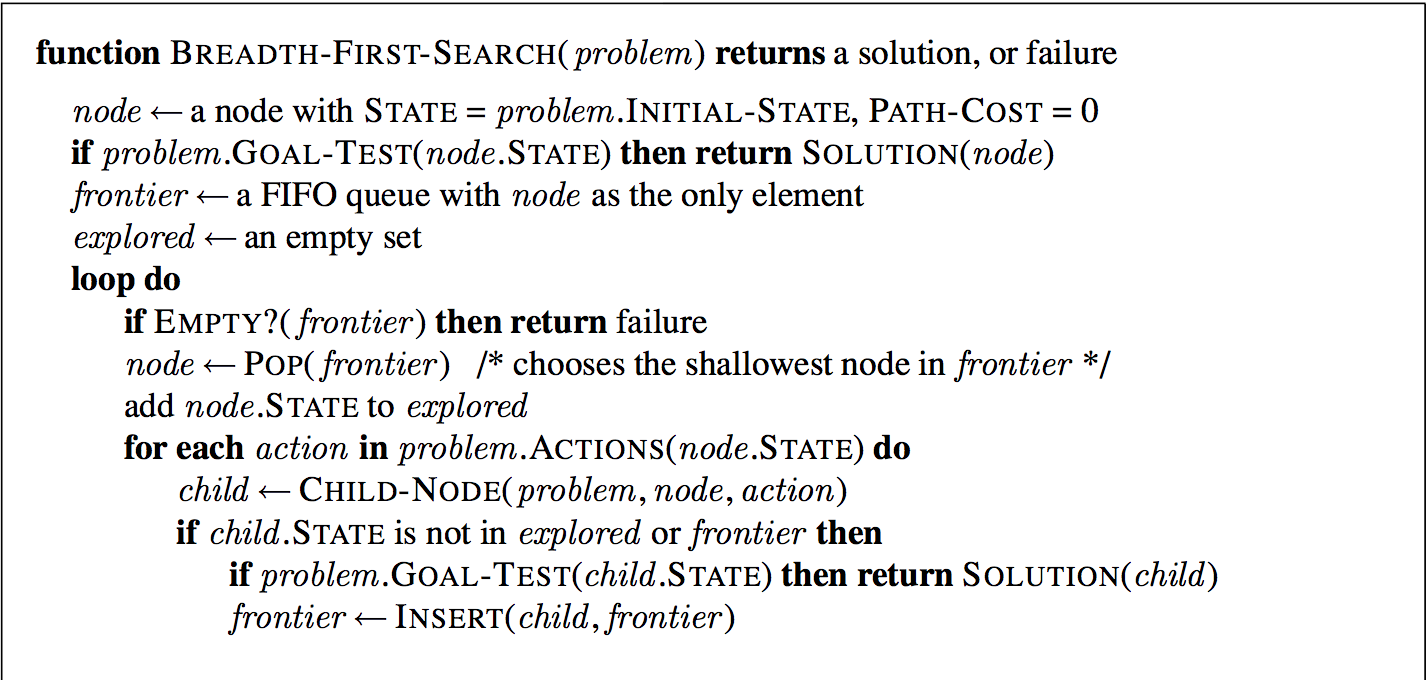
\includegraphics[width=\linewidth]{bfs.png}
  \caption{Breadth-First Search.}
  \label{fig:bfs}
\end{figure}
BFS is \emph{complete} - if the shallowest goal node is at some finite depth
BFS will eventually find it after generating all the shallower nodes. Note
that the \emph{shallowest} is not always the \emph{optimal} one. BFS is only 
optimal if the path cost is a non-decreasing function of the depth of the node.
The time complexity of BFS is:
\begin{equation}
    b + b^2 + b^3 + ... + b^d = O(b^d)
\end{equation}
For the space complexity there will be \(O(b^{d-1})\) nodes in the explored set 
and \(O(b^{d})\) nodes in the frontier, giving space complexity as \(O(b^{d})\).
\emph{Memory requirements are a bigger problem for BFS than execution time and
time is still a major factor. Exponential-complexity search problems cannot
be solved by uninformed methods for any but the smallest instances.}

\subsubsection{Uniform-Cost Search}
This is similar to BFS, but it expands the node with the lowest path cost, the
goal test is applied to a node \emph{not when it's generated, but when it's
chosen for expansion} and a test is added in case a better path is found to a
node currently on the frontier. The algorithm is given in figure \ref{fig:ucs}.
First, we note that whenever this algorithm selects a node for expansion, the 
optimal path to that node is found and second, paths never get shorter as
nodes are added. Thus, \emph{uniform-cost search expands nodes in order of 
their optimal path cost.} This search is complete given that the cost of every
step exceeds some small positive constant \(\epsilon\). The space and time
complexity is \(O(b^{1+\lfloor C^*/\epsilon \rfloor})\), where \(C^*\) is the
cost of the optimal solution.
\begin{figure}
  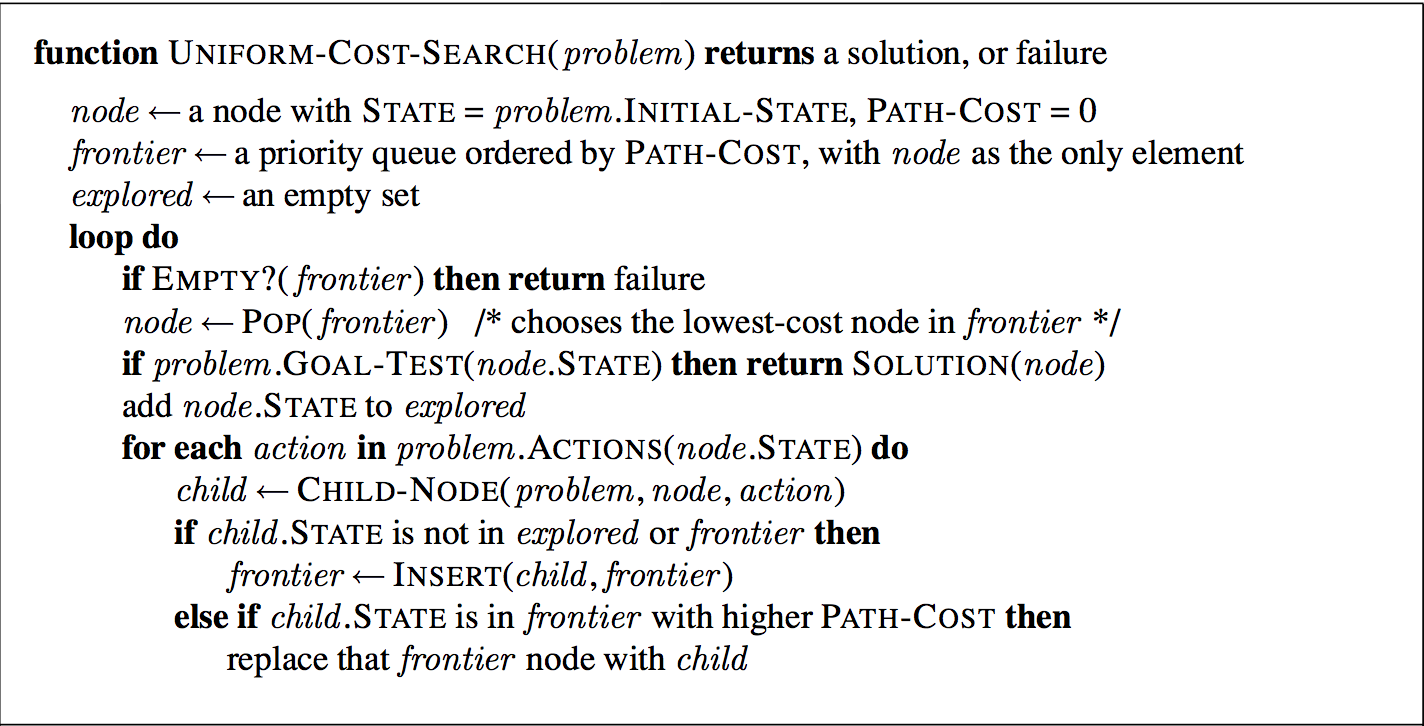
\includegraphics[width=\linewidth]{uniform.png}
  \caption{Uniform-Cost Search.}
  \label{fig:ucs}
\end{figure}
\subsubsection{Depth-First Search}
Depth-First Search always expands upon the deepest node in the frontier, this
is accomplished using a LIFO queue. The graph-search version of the algorithm
is complete in finite spaces but the tree-search version could potentially
fall into a infinite loop. Although, it must be noted that both versions fail
if there is an infinite state space, with an infinite non-goal path e.g.
Knuth's 4 problem. Both versions are also not optimal. The time complexity of
DFS is \(O(b^m)\) and space complexity is \(O(bm)\).
\begin{figure}
  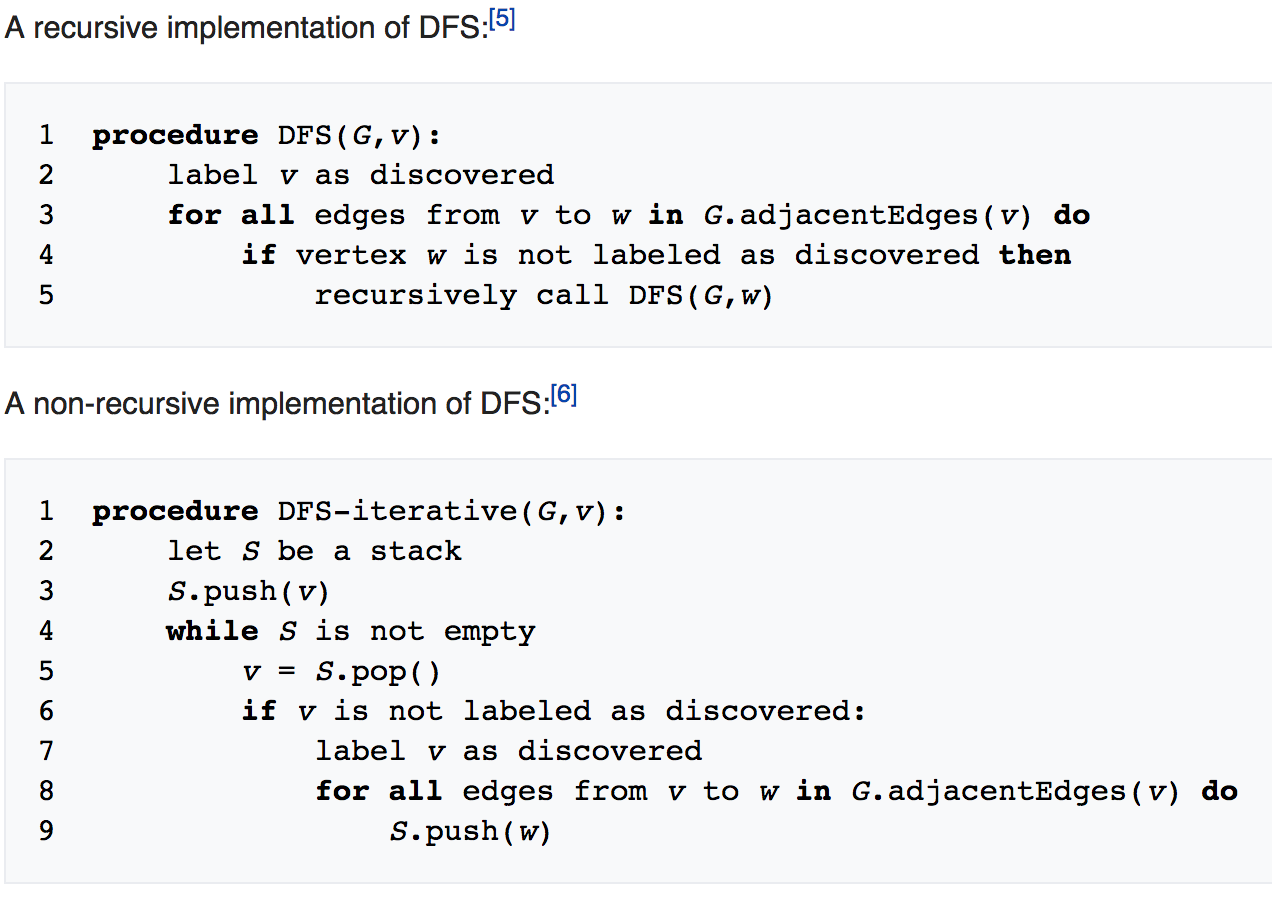
\includegraphics[width=\linewidth]{dfs.png}
  \caption{Depth-First Search.}
  \label{fig:dfs}
\end{figure}
\subsubsection{Depth-Limited Search}
The problem of DFS failing in infinite spaces can be solved if we apply a
limit \(\ell\) to the depth we expand up till. Although, it introduces 
incompleteness if we choose \(\ell < d\) and non-optimality if \(\ell > d \). Its 
time complexity is \(O(b^\ell)\) and its space complexity is \(O(b\ell)\). Its 
pseudocode is shown in figure \ref{fig:dls}.
\begin{figure}
  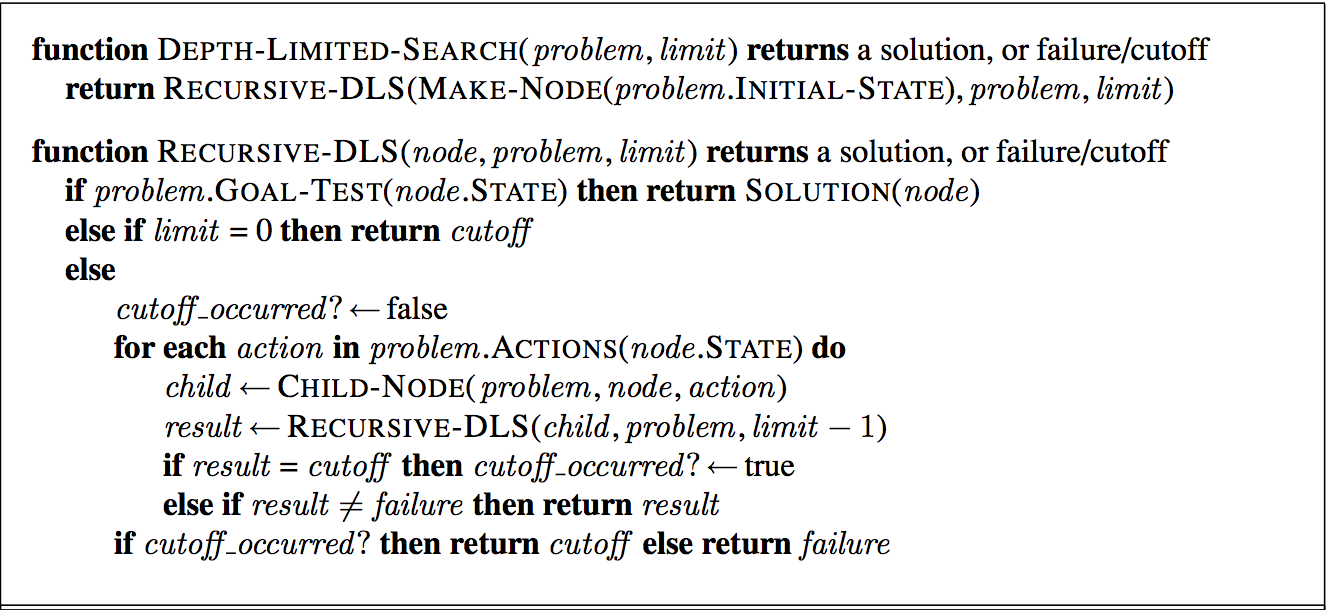
\includegraphics[width=\linewidth]{dls.png}
  \caption{Depth-Limited Search.}
  \label{fig:dls}
\end{figure}
\subsubsection{Iterative Deepening Search}
The algorithm of IDS is shown in figure \ref{fig:ids}. Its space complexity
is \(O(bd)\). Like BFS, IDS is complete if the branching factor is finite and
it is optimal when the path cost is a non-decreasing function of the depth.
The time complexity is:
\begin{equation}
    (d)b + (d - 1)b^2 + ... + (d - d + 1)b^d = O(b^d)
\end{equation}
\emph{In general, IDS is preferred if the search space is large and the depth
of the solution is not known.}
\begin{figure}
  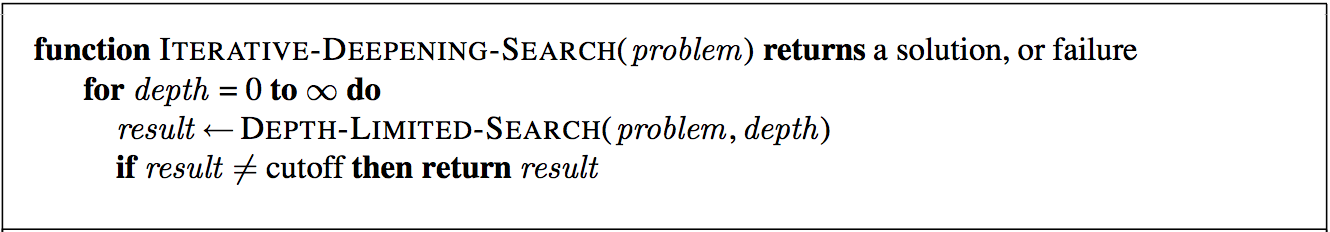
\includegraphics[width=\linewidth]{ids.png}
  \caption{Iterative Deepening Search.}
  \label{fig:ids}
\end{figure}
\subsubsection{Bidirectional Search}
Bidirectional search applies the idea of starting two searches: one from the
initial state and one from the goal state, hoping that they meet in the middle;
with the motivation that \(b^{d/2} + b^{d/2} < b^d\). Thus the space and time
complexity for this algorithm is \(O(b^{d/2})\).
\subsubsection{Comparison of Uninformed Search Strategies}
Figure \ref{fig:comparison} shows comparisons for tree search versions of the 
algorithms discussed. For graph searches, the main difference is that DFS is
complete for finite state spaces and that the space and the time complexities
are bounded by size of the state space.
\begin{figure}
  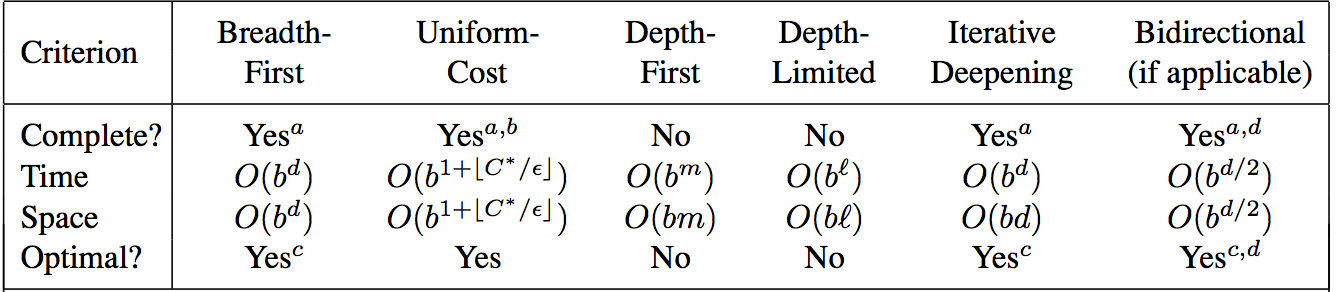
\includegraphics[width=\linewidth]{comparison.png}
  \caption{Comparison of uninformed search strategies. \(b\) is the branching 
  factor; \(d\) is the depth of the shallowest solution; \(m\) is the maximum depth 
  of the search tree; \(l\) is the depth limit. Superscript caveats are as follows:
  \(^a\) complete if \(b\) is finite; \(b\) complete if step costs \(\geq \epsilon\)
   for positive \(\epsilon\); \(^c\) optimal if step costs are all identical; 
  \(^d\) if both directions use breadth-first search.}
  \label{fig:comparison}
\end{figure}

\section{Informed Search Algorithms}
An informed search strategy is one that uses problem-specific knowledge beyond
the definition of the problem itself. The general approach considered is an
instance of a general graph or tree search in which a node is chosen for 
expansion based on its \textbf{evaluation function}, \(f(n)\). Most best-first
algorithms include as a component of \(f\) a \textbf{heuristic function},
denoted by \(h(n)\), which is an estimated cost of the cheapest path from
the state at node \(n\) to a goal state. We use the constraint that if \(n\)
is the goal node then \(h(n) = 0\).
\subsection{Greedy Best-First Search}
This algorithm uses \(f(n) = h(n)\). Due to its greedy nature it is not 
optimal and is also incomplete even in a finite state space, like DFS. The graph
version of this algorithm is complete in finite spaces, but not infinite ones.
The worse case space and time complexity for the tree version is \(O(b^m)\),
where \(m\) is the maximum depth of the search tree.
\subsection{A* Search}
This search evaluates nodes by using:
\begin{equation}
        f(n) = g(n) + h(n)
\end{equation}
Since \(g(n)\) gives the path cost from the start node to node \(n\), and 
\(h(n)\) is the estimated cost of the cheapest path from \(n\) to the goal,
\(f(n)\) is the estimated cost of the cheapest solution through \(n\). Provided 
\(h(n)\) satisfies certain conditions, it's both complete and optimal.
\subsubsection{Conditions for Optimality: Admissibility and Consistency}
The first condition we require is \(h(n)\) be an \textbf{admissible heuristic},
meaning it is one that \emph{never overestimates} the cost to reach the goal.
Thus we have that \(f(n)\) never overestimates the true cost of a solution along
the current path through \(n\). The second condition required is 
\textbf{consistency}, or \textbf{monotonicity} for applications of A* to graph
search. A heuristic \(h(n)\) is consistent if:
\begin{equation}
        h(n) \leq c(n,a,n') + h(n')
\end{equation}
Where \(n'\) is the successor of \(n\) generated by action \(a\). This is a form
of the general \textbf{triangle inequality}, which says that each side of a 
triangle can't be longer than the sum of the other two sides. Here the triangle
is formed by \(n, n'\) and the goal \(G_n\) closest to \(n\).
\subsubsection{Optimality of A*}
We know that \emph{the tree-search version of A* is optimal if \(h(n)\) is 
admissible, while the graph-search version is optimal if \(h(n)\) is consistent.}
First let us establish: \emph{if \(h(n)\) is consistent then the values of
\(f(n)\) along any path are non-decreasing.} Suppose \(n'\) is a successor of
\(n\); then \(g(n') = g(n) + c(n,a,n')\) thus we have:
\begin{equation}
        f(n') = g(n') + h(n') = g(n) + c(n,a,n') + h(n') \geq g(n) + h(n) = f(n)
\end{equation}
The next step is to prove that \emph{whenever A* selects a node for expansion,
the optimal path to that node has been found.} The fact that \(f\) costs are
non-decreasing along any path allows us to draw \textbf{contours} in the state
space. If \(C^*\) is the cost of the optimal solution path, then:
\begin{itemize}
        \item A* expands all nodes with \(f(n) < C^*\).
        \item A* might then expand some of the nodes right on the ``goal contour''
              (where \(f(n) = C^*)\) before selecting the goal node.
\end{itemize}
Completeness requires that there be only finitely many nodes wih cost less than
or equal to \(C^*\), a condition only met if all step costs exceed some finite
\(\epsilon\) and if \(b\) is finite. One final observation is A* is 
\textbf{optimally efficient} for any given consistent heuristic i.e. no other
optimal algorithm is guaranteed to expand fewer nodes than A* because any 
algorithm that doesn't expand all nodes with \(f(n) < C^*\) runs the risk of 
missing the optimal solution. The space complexity is \(O(b^d)\) and the 
time complexity is \(O(b^\Delta)\), with 
\(\Delta \equiv h^* - h\) which is the \textbf{absolute error}.
For constant depth we have \(O(b^{\epsilon d})\), with 
\(\epsilon \equiv (h^* - h)/h^*\) which is the \textbf{relative error}.
\subsection{Heuristic Functions}
There are a few good heuristics used for the 8-puzzle like the number of 
misplaces tiles and the \textbf{manhattan distance} which is the sum of 
horizontal and vertical distances. One way to characterize the quality of 
a heuristic is the \textbf{effective branching factor}, \(b^*\). If the total
number of nodes generated by A* for a particular problem is \(N\), and the 
solution depth is \(d\), then \(b^*\) is the branching factor that a uniform
tree of depth \(d\) would have in order to contain \(N + 1\) nodes. Thus:
\begin{equation}
        N + 1 = 1 + b^* + (b^*)^2 + ... + (b^*)^d
\end{equation}
If \(\forall\) nodes \(n, h_2(n) \geq h_1(n) \implies h_2\) \textbf{dominates} \(h_1\).
\subsubsection{Relaxed Problems}
A problem with fewer restrictions on the actions is called a \textbf{relaxed 
problem}. The state-space graph of the relaxed problem is a \emph{supergraph}
of the original state space because the removal of restrictions creates added
edges in the graph. Because edges are added to the state-space, any optimal
solution in the original problem is also a solution in the relaxed problem,
but the relaxed problems may have better solutions. Hence, \emph{the cost of 
an optimal solution to a relaxed problem is an admissible heuristic for the
original problem.} Furthermore, because the derived heuristic is an exact cost
for the relaxed problem, it muse obey the triangle inequality and is therefore 
consistent. If the relaxed problem is hard to solve, then the values of the 
corresponding heuristic will be expensive to compute. Since a collection of 
admissible heuristics are obtained, we can use an appropriate heuristic
on each node individually using:
\begin{equation}
        h(n) = \max\{h_1(n), ... , h_m(n)\}
\end{equation}
\subsection{Local Search Algorithms}
These algorithms operate using a single \textbf{current node} and generally
move only to neighbors of that node and the paths followed aren't retained.
Thus they have the advantages:
\begin{itemize}
        \item They use very little memory - usually a constant amount
        \item They can often find reasonable solutions in large or infinite
                state spaces
\end{itemize}
\subsubsection{Hill-Climbing Search}
The algorithm is shown in figure \ref{fig:hill}. It is comparative to ``trying
to find the top of Mount Everest in a thick fog while suffering from amnesia''.
It is also called \textbf{greedy local search}. Hill-Climbing gets stuck in
\textbf{local maxima/minima, ridges} and \textbf{plateaux}.
\begin{figure}
  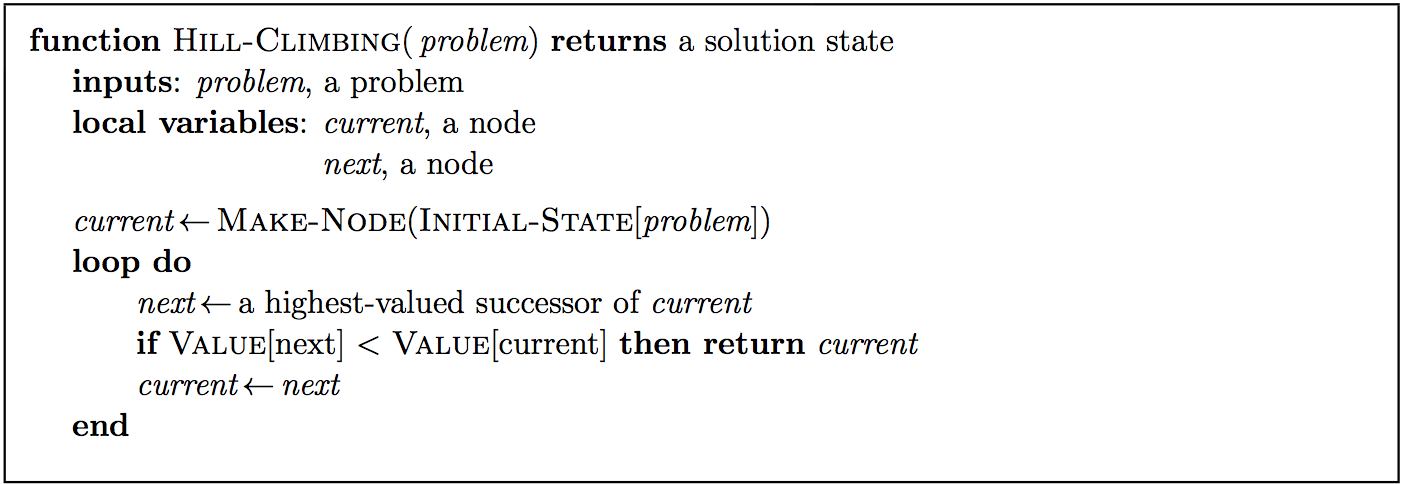
\includegraphics[width=\linewidth]{hill.png}
  \caption{Hill-Climbing Search.}
  \label{fig:hill}
\end{figure}
\section{Adversarial Search}
A \textbf{utility function} is defined as the final numeric value for a game
that ends in terminal state \(s\) for a player \(p\). A \textbf{zero-sum game}
is defined as one where the total payoff to every player is the same in 
every instance of the game.
\subsection{The Minimax Algorithm}
The algorithm is shown in figure \ref{fig:minimax}. The utility values of the 
leaf nodes are computed and the corresponding minimax values are backed up
the tree recursively. The time complexity of this algorithm is \(O(b^m)\), where
\(m\) is the maximum depth of the tree and there are \(b\) legal moves at each
point. The space complexity is \(O(bm)\) for an implementation that generates
all the actions at once and \(O(m)\) for an implementation that generates 
actions one at a time.
\begin{figure}
  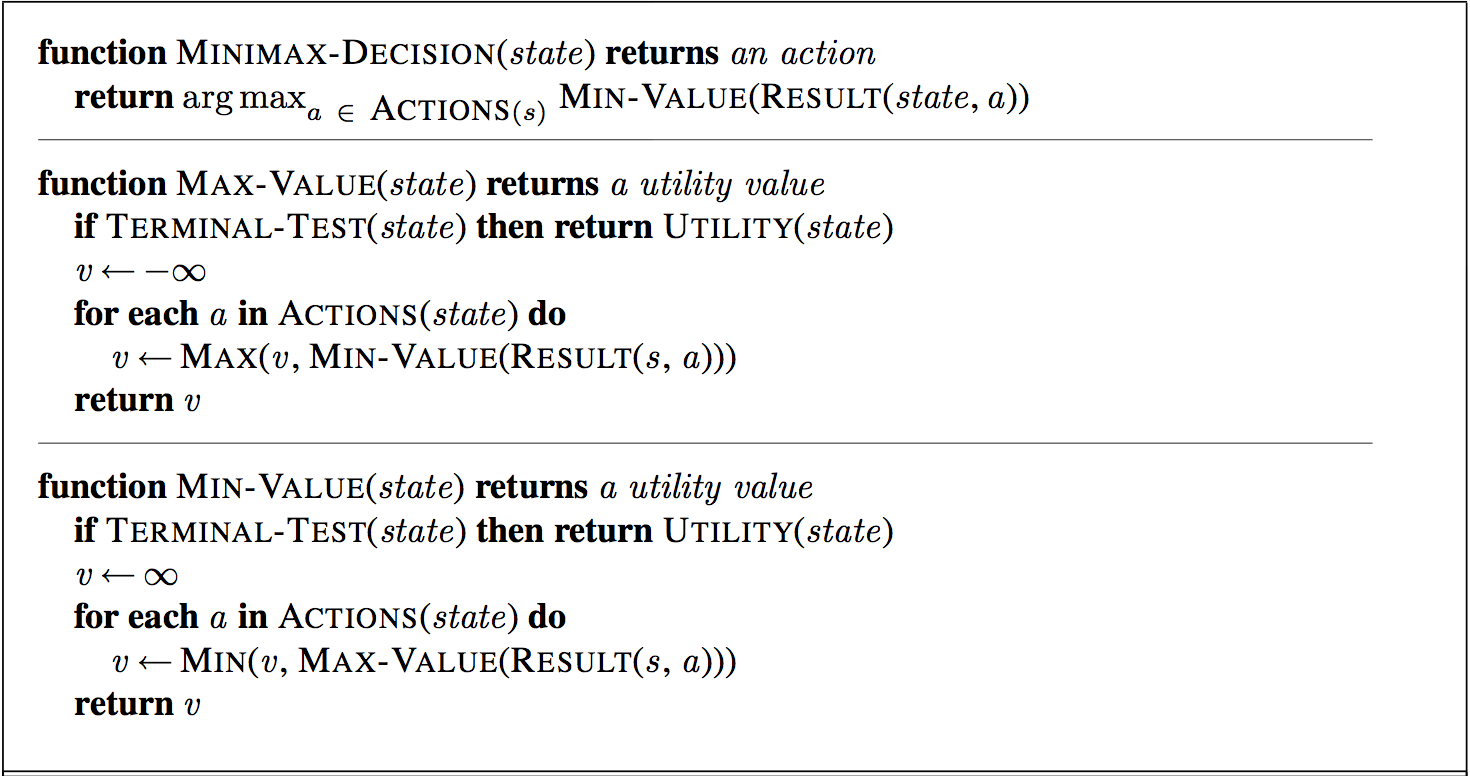
\includegraphics[width=\linewidth]{minimax.png}
  \caption{The Minimax Algorithm.}
  \label{fig:minimax}
\end{figure}
\subsection{Alpha-Beta Pruning}
A way to improve the abysmal complexity of Minimax is to use alpha-beta 
pruning, which prunes away branches that can't possibly influence the final
decision. \(\alpha\) is the best choice we have found so far for Max and 
\(\beta\) is the best choice for Min. The algorithm is applied in figure
\ref{fig:alpha-beta}. \textbf{Move ordering} can be applied to improve
complexity to \(O(b^{m/2})\) and the branching factor becomes \(\sqrt{b}\). If the 
successors are examined at random and not best-first the complexity increases
to \(O(b^{3m/4})\). The best moves in a game are called \textbf{killer moves}
and a killer move heuristic is used to find them. The hash table of 
previously seen moves is called a \textbf{transposition table}.
\begin{figure}
  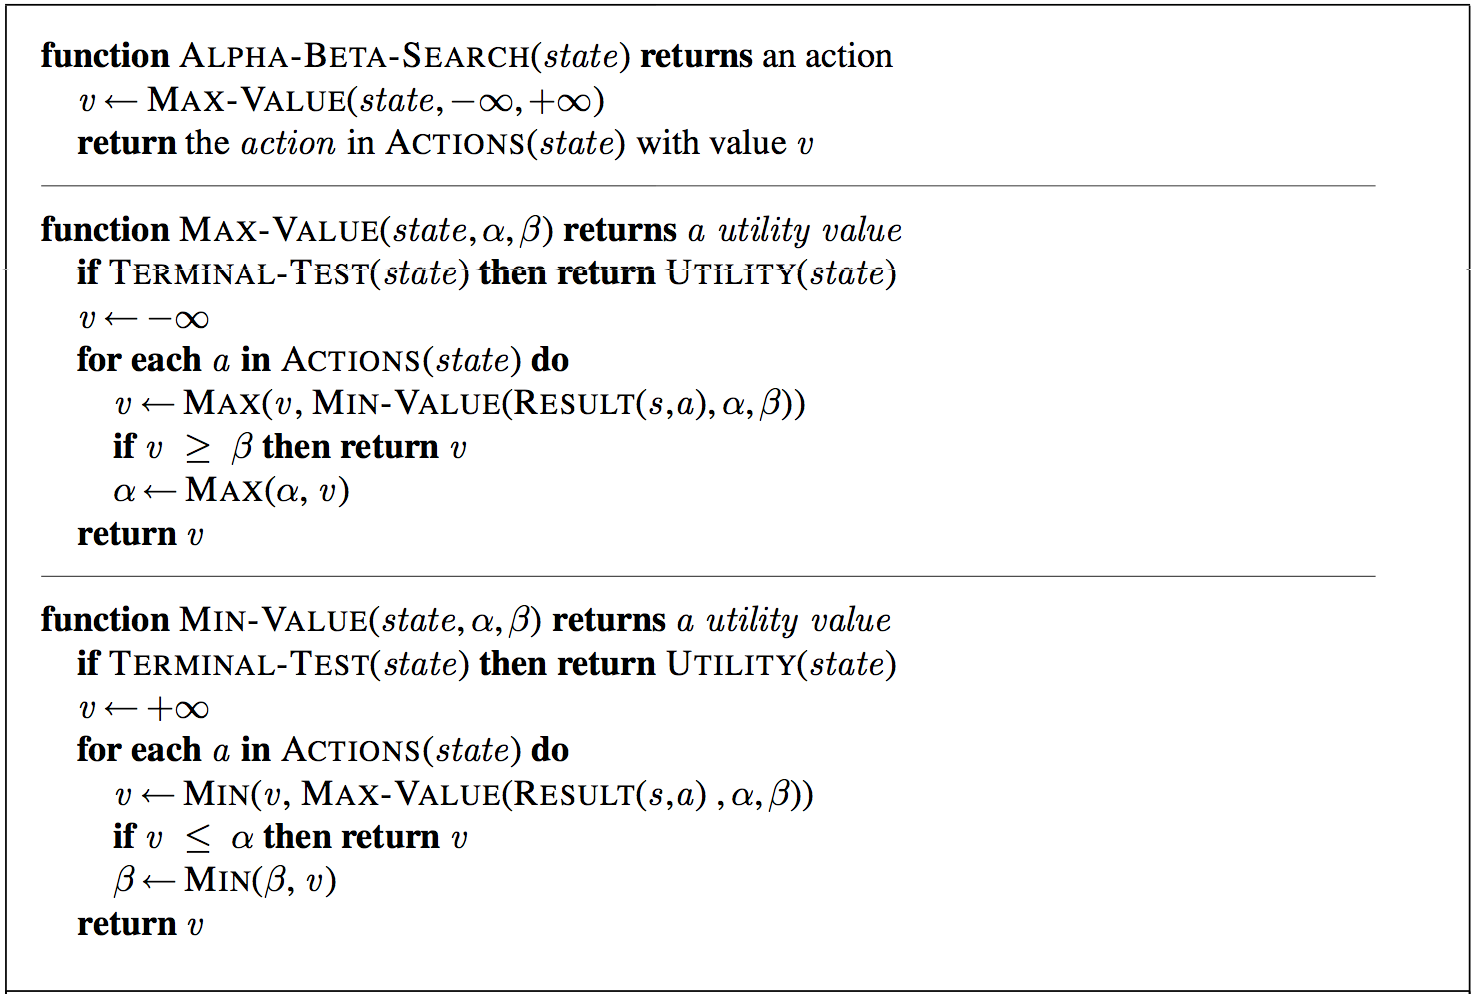
\includegraphics[width=\linewidth]{alpha-beta.png}
  \caption{Alpha-Beta Pruning.}
  \label{fig:alpha-beta}
\end{figure}
\subsection{Evaluation Functions}
An evaluation function returns an estimate of the expected utility from a given
position. This is useful as sometimes we want to stop our search at a depth 
limit and evaluate the leaf nodes using this function. Most evaluation
functions compute separate numerical contributions from each feature then
combine them to find the total value. These types of functions are also called
\textbf{weighted linear functions} because:
\begin{equation}
        E(s) = w_1f_1(s) + w_2f_2(s) + ... + w_nf_n(s) = \sum_{i=1}^{n} w_if_i(s)
\end{equation}
In \textbf{cutting off search} \texttt{isTerminal} and \texttt{utility} in minimax
are replaced by \texttt{cutoff} and \texttt{eval}. In stochastic games, 
chance nodes are added in addition to min/max nodes. The minimax values are also
replaced by \textbf{expected values}: the average over all possible outcomes of 
the chance nodes. This leads us to make \textbf{expecti-minimax} for games with
chance nodes.
\end{document}